% Benchmark: PCPOP vs OSCAR
\documentclass[11pt]{article}
\usepackage[utf8]{inputenc}
\usepackage[T1]{fontenc}
\usepackage{lmodern}
\usepackage{graphicx}
\usepackage{caption}
\usepackage{subcaption}
\usepackage[a4paper,margin=1in]{geometry}
\usepackage{microtype}
\usepackage{float}
\usepackage{hyperref}

\title{Benchmark PCPOP vs OSCAR}
\author{Abhishek Mishra}
\date{\today}

\begin{document}
\maketitle

\section{Introduction}

The equality constraints in a polynomial optimization can be leveraged to reduce the SDPs sizes. This requires finding normal forms under the equalities. PCPOP and OSCAR follow different approaches but both have two distinct phases. First called startup phase where OSCAR computes a Grobner Basis and PCPOP build the quotient monoid structure. The second phase is the reduction phase where both systems reduce monomials/polynomials to their normal forms. Here we will consider the example of partial commutations where some pairs of variables commute and some not. For a level d relaxation, OSCAR needs to compute the Grobner basis up to degree 2d while PCPOP builds the Partially commutative monoid structure once and can reduce monomials of any degree or any level. This makes PCPOP better atleast for qualities including partial commutations and binomial constraints (projectors, unitary \dots).

\section{Example1: Partial Commutations}

Here we will consider set of variables $V = \{x_1, x_2, \ldots, x_{3*n}\}$ where the variables $V$ can be partitioned into 3 groups of n variables each say $A=\{x_1,x_2 \ldots x_n\}$, $B=\{x_{n+1},x_{n+2} \ldots x_{2*n}\}$ and $C=\{x_{2*n+1},x_{2*n+2} \ldots x_{3*n}\}$. Every variable in group A commutes with every variable in group B  and every variable in group B commutes with every variable in group C. However, no variable in group A commutes with any variable in group C. For all the compairion plots, at low levels one can see the plots coincide but there is a big gap still.
\begin{figure}[H]
	\centering
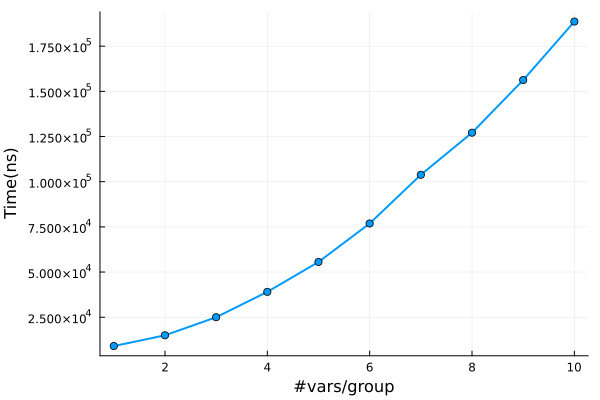
\includegraphics[width=0.8\textwidth]{plots/benchmark1/startup/M.png}
\caption{Time PCPOP takes to build the partially comm. monoid where X axis is n i.e number of variables in each of three group.}
\end{figure}

\begin{figure}[H]
	\centering
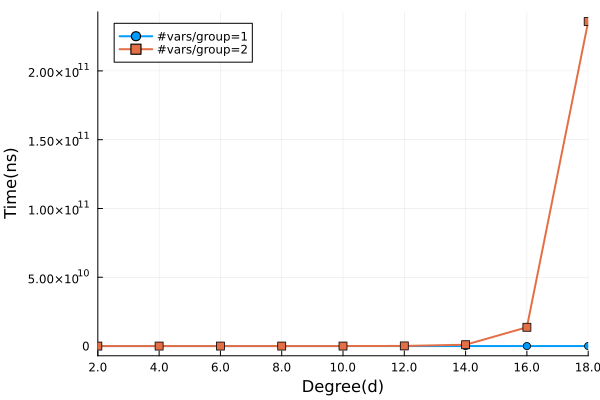
\includegraphics[width=0.8\textwidth]{plots/benchmark1/startup/g_vars1vs2.png}
\caption{Time OSCAR takes to compute the GB for degree upto level*2. Here the number of variables in each group is 1 for blue plot and 2 for orange.}
\end{figure}

\begin{figure}[H]
	\centering
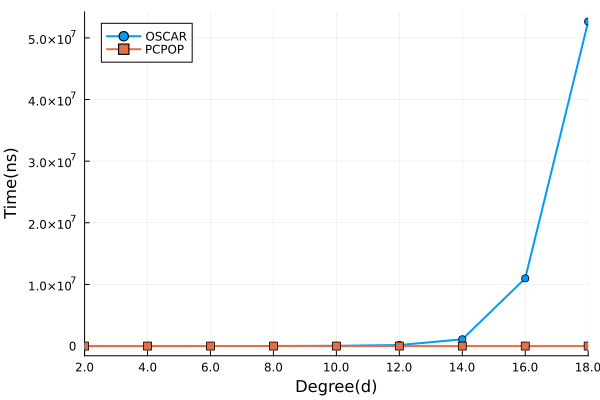
\includegraphics[width=0.8\textwidth]{plots/benchmark1/normal_form/OSCARvsPCPOP_vars=2.png}
\caption{Example1: Comparision of PCPOP vs OSCAR. Here the number of variables in each group is 2. A random monomial m of degree "level" is generated and the time taken to reduce m*m to its normal form is recorded. OSCAR uses $normal\_form(m*m,gb)$ where gb is the Grobner basis computed upto degree $level*2$ but PCPOP handles normal form implicitly.}
\end{figure}

\section{Example2: Partial Commutations with projectors}

In this example we have same variables and commutations as before but in addition all the variables $x_i$ are projectors i.e $x_i^2 = x_i$.

\begin{figure}[H]
	\centering
\includegraphics[width=0.7\textwidth]{plots/benchmark2/normal_form/OSCARvsPCPOP_vars=1.png}
\caption{Example2: Comparision of PCPOP vs OSCAR. Here the number of variables in each group is 1. A random monomial m of degree "level" is generated and the time taken to reduce m*m to its normal form is recorded.}
\end{figure}

\begin{figure}[H]
	\centering

\includegraphics[width=0.8\textwidth]{plots/benchmark2/normal_form/OSCARvsPCPOP_vars=2.png}
\caption{Example2: Comparision of PCPOP vs OSCAR. Here the number of variables in each group is 2. A random monomial m of degree "level" is generated and the time taken to reduce m*m to its normal form is recorded.}
\end{figure}

\end{document}
